% ------- textdoclet_include/finish.tex



\section{verwendetes Datenbankschema}
Das System persistiert Daten in einer zentralen MySQL-Datenbank auf dem Tomcat-Server und zusätzlich auf einer lokalen SQLite-Datenbank auf den Clients. Beide Datenbanken verwenden das gleiche Schema.\\


\section{Klassendiagramme}

\section{Sequenzdiagramme}

\subsection{Hinzufügen eines Gruppenmitglieds}

\begin{figure}[H]
	\centering
	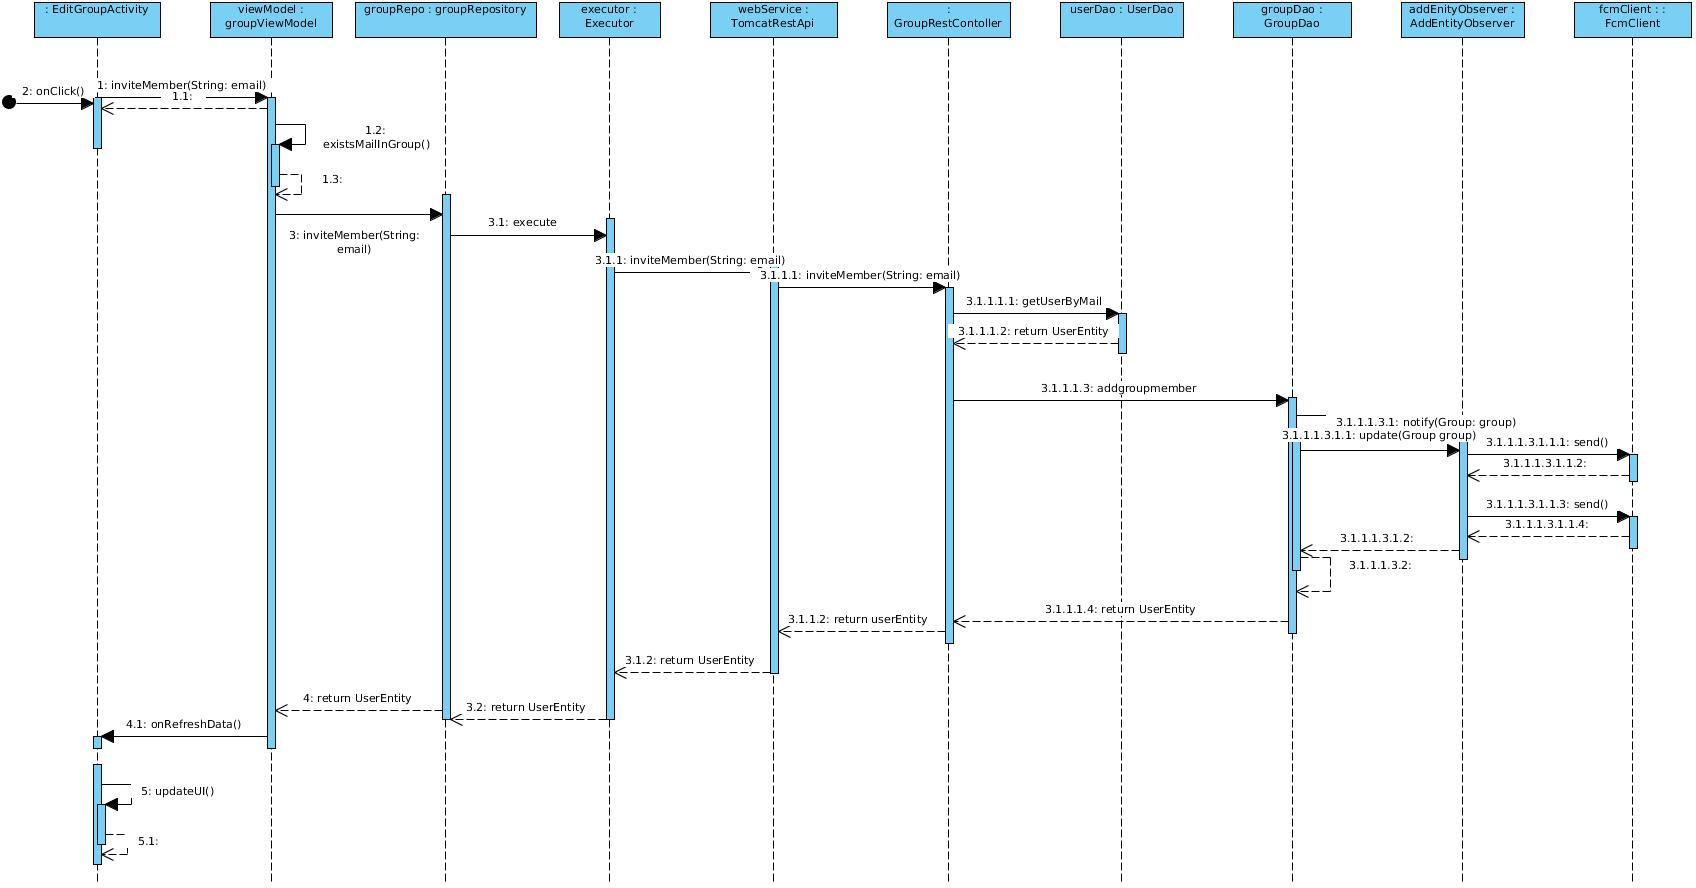
\includegraphics[width=1\textwidth]{../Sequenzdiagramme/addGroupMember.jpg}
	\caption{Sequenzdiagramm - Hinzufügen eines Gruppenmitglieds Teil 1}
\end{figure}

Das obige Sequenzdiagramm zeigt, was während der Ausführung des Programms passiert, wenn ein Benutzer die Funktion "inviteMember" ausführt. Das User Interface stellt dem Benutzer ein Textfeld zur Eingabe der E-Mailadresse und einen Button zum Bestätigen zur Verfügung. Bei Klick dieses Buttons extrahiert die Activity-Klasse die eingegebene Mail-Adresse aus dem Textfeld und übergibt diese an das ViewModel über den Methodenaufruf "inviteMember". Das ViewModel überprüft zunächst ob es bereits einen Benutzer in Gruppe gibt, der diese E-Mailadresse besitzt. Falls nicht, wird die Gruppeneinladung an die Grouprepository weitergeleitet und von dort über die Klasse TomcatrestApi an den Server gesendet.

Empfängt der Server eine Anfrage, einen User zu einer Gruppe hinzuzufügen, wird diese Anfrage zunächst an das UserDao weitergegeben. Dort wird zuerst die Methode getUserByMail() aufgerufen, um den richtigen Benutzer aus der Datenbank zu finden. Danach wird die addGroupmember-methode des GroupDaos aufgerufen. In dieser methode wird die neue gruppenanfrage in der Datenbank gespeichert und es werden die Observer benachrichtigt, dass sich Daten geändert haben.

Der AddEntityObserver erkennt, dass es sich um eine Änderung handelt, die seinen Veratnwortlichkeitsbereich betrifft. Er bekommt beim Aufruf der update()-Methode die Gruppe mit der zusätzlichen Gruppenanfrage übergeben. Der Observer extrahiert alle Gruppenmitglieder aus dem Gruppenobjekt und ruft die send()-methode des FcmClients auf, um das geänderte Gruppenobjekt an alle Gruppenmitglieder zu senden. Danach wird die send()-Methode ein zweites Mal aufgerufen, um dem neuen Gruppenmitglied die neue Gruppenanfrage zu übermitteln.

\begin{figure}[H]
	\centering
	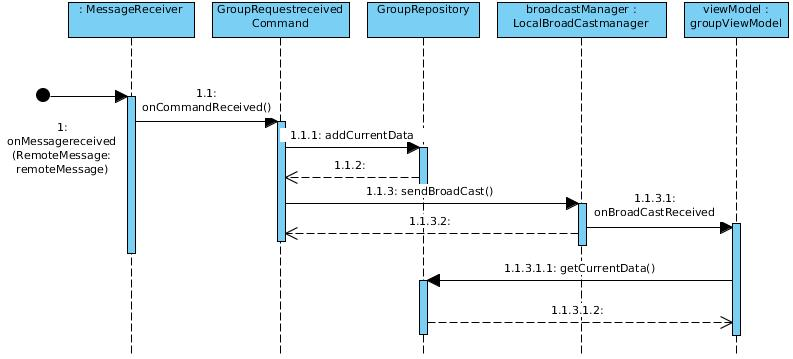
\includegraphics[width=1\textwidth]{../Sequenzdiagramme/addMember2.jpg}
	\caption{Sequenzdiagramm - Hinzufügen eines Gruppenmitglieds Teil 2}
\end{figure}

Das zweite Sequenzdiagramm zeigt, was passiert, wenn an einen Benutzer eine Gruppenmitgliedschaftsanfrage gesendet wird. Die Nachricht, die von dem Server, über dem Firebase Cloud Messaging Server, an den Client gesendet wird, löst einen Aufruf der Methode onMessageReceived() in der Klasse MessageReceiver aus. Diese Klasse extrahiert das JSON-Feld COMMAND\_CODE aus dem empfangenen JSON-Objekt und findet so heraus, an welches ServerCommand-Objekt die Anfrage weitergeleitet werden muss.

Nach Weiterleitung der Anfrage an den GroupRequestReceivedCommand wird dort das Datenfeld aus der JSON-Nachricht extrahiert. dort ist die Gruppe gespeichert, zu der er Benutzer eingeladen wurde. Diese Gruppe wird in dem öffentlichen "CurrentData" Field des GroupRepository gespeichert. Danach schickt das GroupRequestReceivedCommand-Objekt einen Broadcast an alle ViewModels. Das GroupViewModel erkennt, dass der Broadcast eine Änderung der Gruppen des Benutzers betrifft. Daher wird dort die onBroadcastReceived()-Methode auferufen. Daraufhin holt sich das ViewModel die aktualisierten Daten von der GoupRepository ab, durch einen Aufruf der getCurrentData()-Methode. Da das UI die LiveData der ViewModels beobachtet, wird automatisch bei einer Aktualisierung des ViewModels auch das UI aktualisiert und zeigt die neuen Daten an.

\subsection{Entfernen einer Gruppe}

\begin{figure}[H]
	\centering
	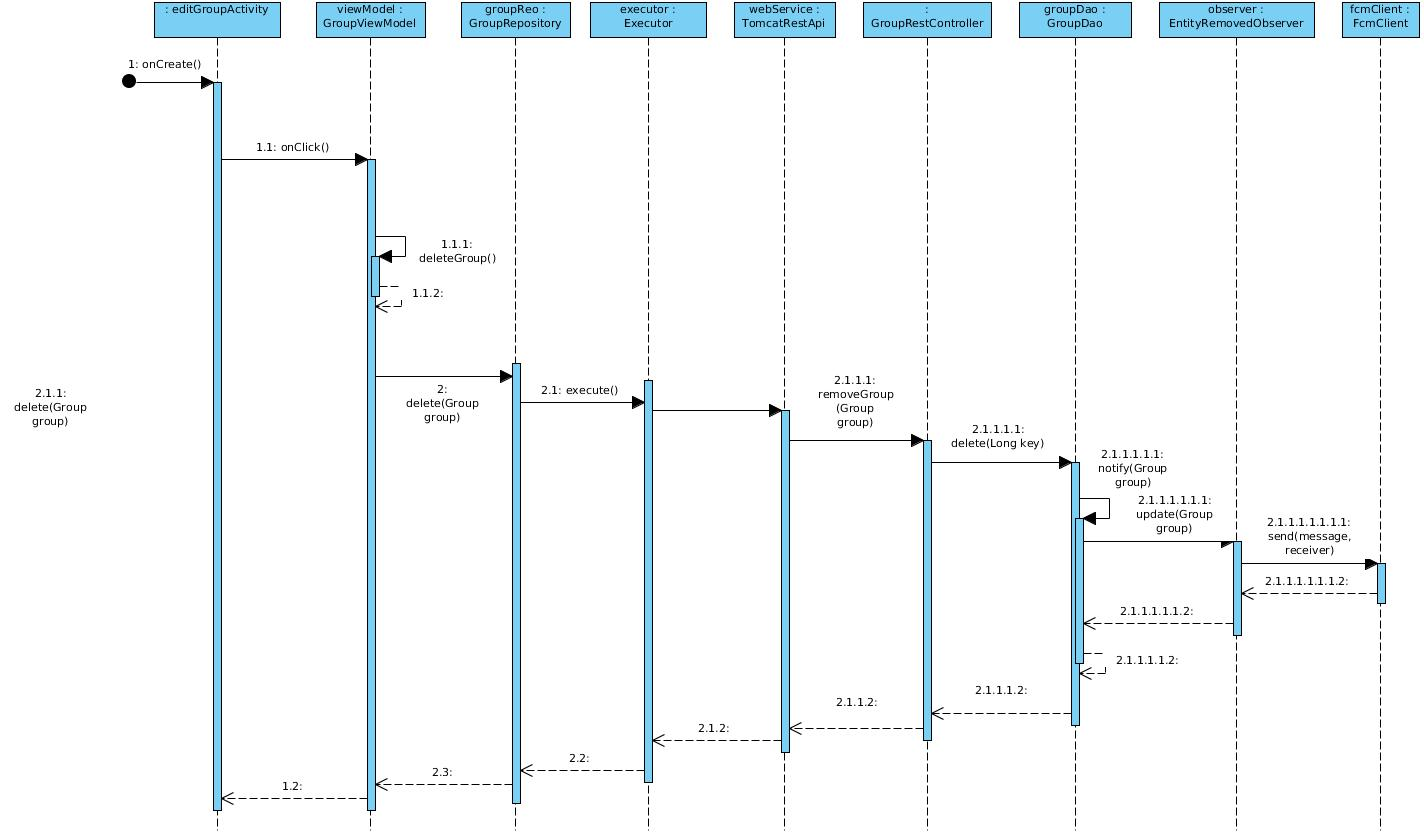
\includegraphics[width=1\textwidth]{../Sequenzdiagramme/deleteGroup_sequenz.jpg}
	\caption{Sequenzdiagramm - Entfernen einer Gruppe}
\end{figure}

Das obige Sequenzdiagramm zeigt den Programmablauf, nachdem ein Benutzer die "Gruppe löschen"-Funktion ausgelöst hat. Das UI gibt den Button Press an das GroupViewModel weiter. Dort wird die Gruppe zunächst in den lokaeln Daten gelöscht. Dabei muss sichergestellt werden, dass die Daten nach dem Löschen konsistent sind, also z.B. auch alle GOs der Gruppe gelöscht wurden.

Danahc wird die Anfrage über die GroupRepository und das Rest API an den Server übergeben, wo sie durch den Methodenaufruf deleteGroup() in der GroupRestController-Klasse ankommt. Von dort aus wird die Anfrage an das GroupDao gegeben, welches die Gruppe in der Datenbank löscht. Auch hier muss auf die Konsistenz der Daten geachtet werden. Danach werden die Observer des GroupDaos benachrichtigt, dass eine Ändeurng stattgefunden hat. Da die Änderung nur den EntityRemovedObserver betrifft, wird bei diesem Objekt die Methode update() aufgerufen. Mit dem Methodenaufruf wird auch die gelöschte Gruppe übergeben.

Der Observer baut ein Message-Objekt aus der erhaltenen Gruppe und extrahiert eine Listse aller Gruppenmitglieder aus dem Gruppenobjekt. Diese Daten werden witergegeben an dem FcmClient über die Methode send(). Dadurch werden die Nachrichten über die Löschung der Gruppe an die Gruppenmitglieder geschickt, damit diese ihre lokalen Daten anpassen können.

\section{Finish}{

}
% ------- textdoclet_include/finish.tex end
